\documentclass[11pt]{article}
\usepackage[margin=0.85in]{geometry}
\usepackage{graphicx}
\usepackage{amsmath}
\title{R99: degree-112 marked-23 lambda resultant norm}
\author{Koblitz modular IC research}
\date{3 November 2026}
\begin{document}
\maketitle
The frozen source-bound Singular attempt computed
$\operatorname{Res}_y(f_{51},\operatorname{Res}_l(G_{51},\partial_lG_{51}))$
for the accepted R51/R63 degree-112 triangular source. Both resultants are
nonzero. The final rational norm has numerator degree 1968, 74 nonzero
terms, and denominator $x^{2608}$. Every numerator exponent is divisible
by 16, suggesting a degree-123 Frobenius root to factor next.

The native run exited zero, printed its exact pass marker, and contained no
Singular error lines. A separate fresh Singular process reproduced the exact
output byte-for-byte. The immutable raw archive contains both runs and has
SHA-256
\texttt{7cebf6664d1442401cc8ba40cde0df109fd29a24c663af6d}\linebreak
\texttt{67b0b5e9cb72caa7}.

\begin{center}
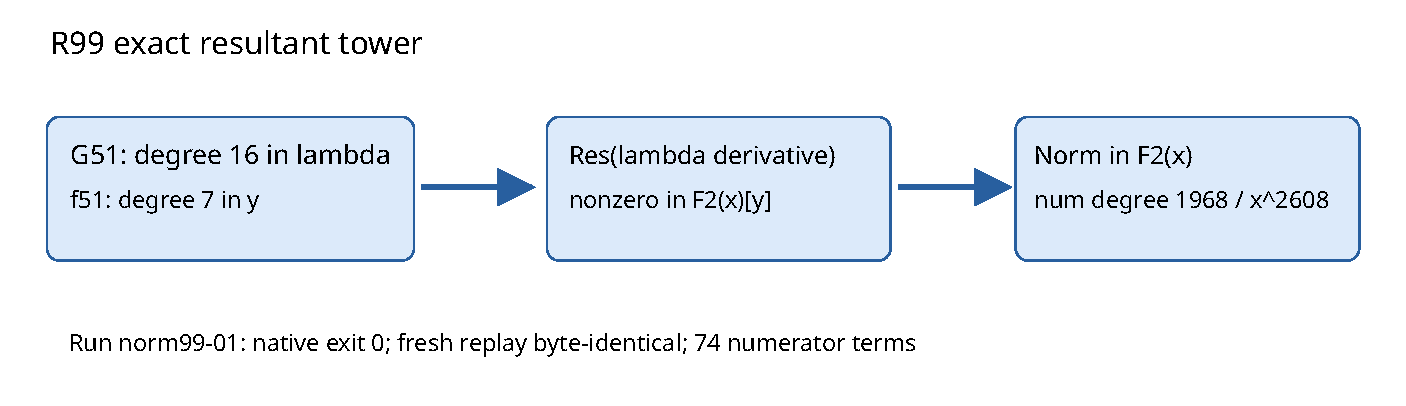
\includegraphics[width=0.97\linewidth]{diagram.pdf}
\end{center}

This calculation gives the lambda derivative norm of the displayed
monogenic order on $D(x)$. Factorization of the degree-123 candidate root,
then local normalization at the combined finite supports and infinity,
are the next steps. No normalized ramification index is inferred here.
\end{document}
